\section{Resultados}

He realizado las pruebas definidas en la sección anterior con 1000 iteraciones y
he pasado los datos por dos \textit{scripts} de R para analizar los datos y
obtener representaciones gráficas de los mismos.

En las siguientes subsecciones se van a presentar los resultados obtenidos de
las 2 pruebas y se van a discutir algunas de sus implicaciones.

\subsection{Tiempo de lanzamiento}

Primero, vamos a ver los resultados de las pruebas de tiempo de lanzamiento.
Estos resultados los encontramos en el cuadro \ref{tab:start-results}. Podemos
apreciar como el tiempo medio de lanzamiento es notablemente superior en i386,
aunque la desviación típica es algo inferior en esta plataforma, indicando que
los tiempos son más consistentes.

\begin{table}[h!]
    \caption{Resultados de las pruebas de tiempo de lanzamiento en milisegundos}
    \label{tab:start-results}
    \begin{center}
        \begin{tabular}{ |c|c|c|c|c|c| }
            \hline
            \textbf{Plataforma} & \textbf{Impl.} & \textbf{Media} &
            \textbf{Desviación} & \textbf{Min}   & \textbf{Max}           \\
            \hline
            arm32v7             & C              & 1693           &
            165                 & 1472           & 2548                   \\
            \hline
            arm32v7             & Go             & 1693           & 163 &
            1445                & 2718                                    \\
            \hline
            arm32v7             & Rust           & 1701           & 156 &
            1478                & 2378                                    \\
            \hline
            i386                & C              & 2606           &
            159                 & 1918           & 3496                   \\
            \hline
            i386                & Go             & 2615           & 156 &
            2010                & 3488                                    \\
            \hline
            i386                & Rust           & 2608           & 148 &
            1961                & 3530                                    \\
            \hline
        \end{tabular}
    \end{center}
\end{table}

Otro aspecto que se aprecia es que no hay diferencias realmente notables entre
las implementaciones en distintos lenguajes, obteniendo todos más o menos los
mismos resultados para una misma plataforma. Esto se puede apreciar aún mejor en
las gráficas de las Figuras \ref{fig:start-time-arm} y
\ref{fig:start-time-i386}. Comparando estas dos gráficas, se puede comprobar que
los tiempos en i386, aunque son más altos, son más estables que los registrados
en arm32v7, tal y como se ha indicado antes.

Para terminar con los resultados de estas pruebas, vemos en la Figura
\ref{fig:start-time-mean} una gráfica comparativa de los tiempos medios.
Confirmamos lo que ya se veía en el cuadro anterior: los tiempos son más bajos
en arm32v7 (en torno a 1.7 segundos frente a los 2.6 de i386) y no hay una
diferencia notable entre los lenguajes usados para implementar el contenedor de
prueba.

\begin{figure}
    \centering
    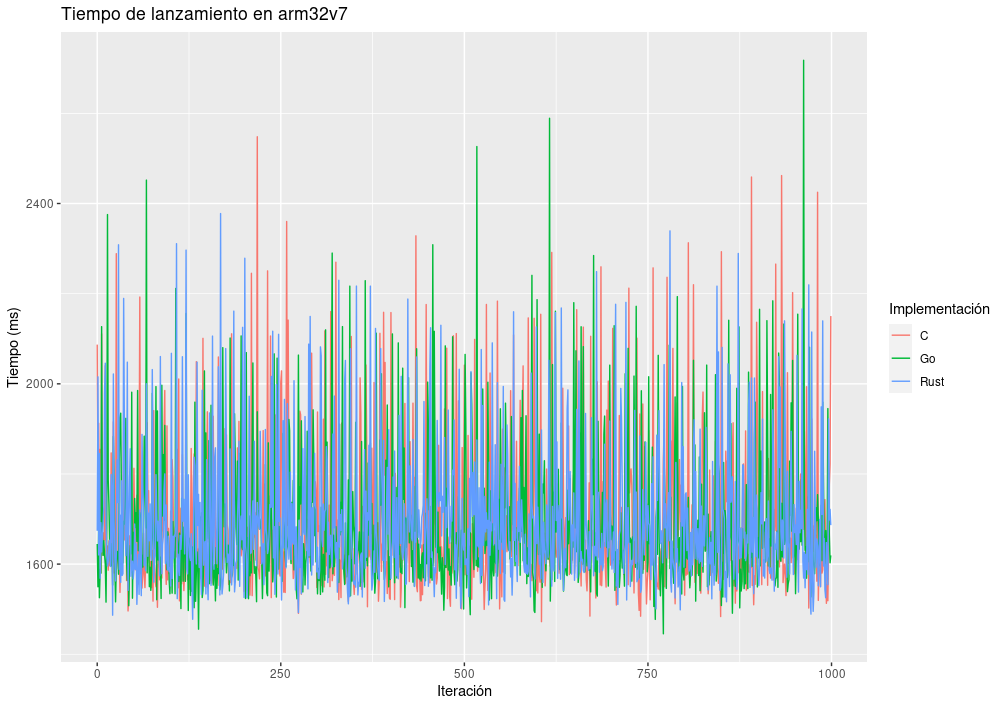
\includegraphics[width=\textwidth]{images/start-time/arm.png}
    \caption{Tiempos de lanzamiento en armv7}
    \label{fig:start-time-arm}
\end{figure}

\begin{figure}
    \centering
    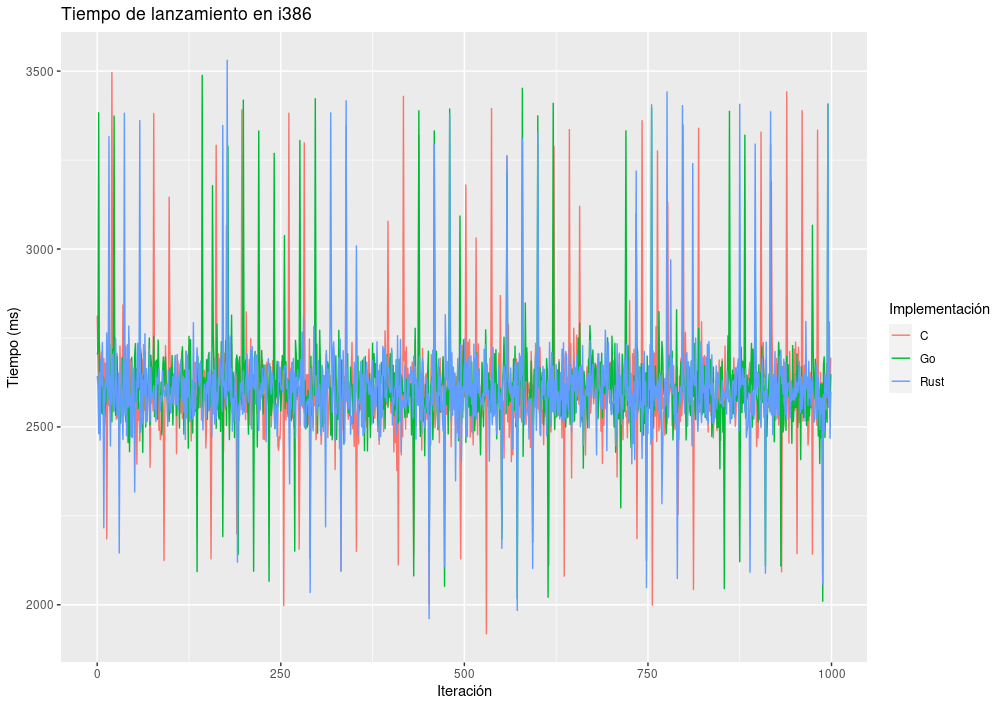
\includegraphics[width=\textwidth]{images/start-time/i386.png}
    \caption{Tiempos de lanzamiento en i386}
    \label{fig:start-time-i386}
\end{figure}

\begin{figure}
    \centering
    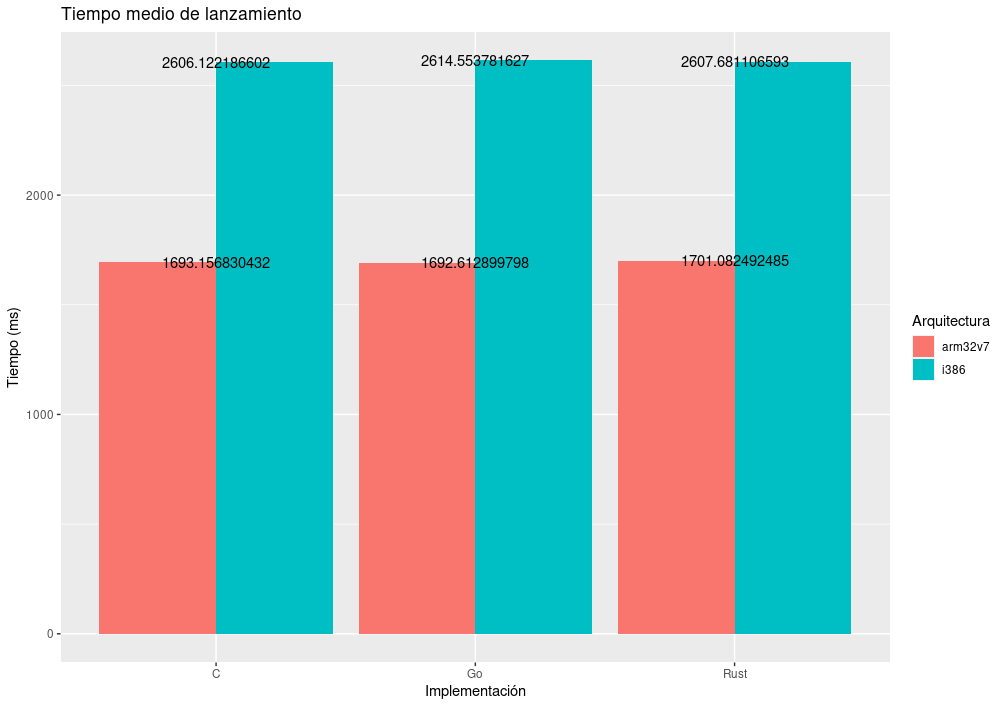
\includegraphics[width=\textwidth]{images/start-time/mean.png}
    \caption{Tiempos de lanzamiento medios en ambas plataformas}
    \label{fig:start-time-mean}
\end{figure}

\newpage

\subsection{Tiempo de respuesta}

En el cuadro \ref{tab:response-results} encontramos los resultados que se han
obtenido para las pruebas del tiempo de respuesta. Al haber tantas combinaciones
posibles de plataforma, versión del proceso maestro y lenguaje de implementación
del contenedor de prueba, se van a ir explicando y analizando los resultados con
varias gráficas para que sea más sencilla su comprensión.

Vamos a comenzar con la plataforma arm32v7. En la Figura
\ref{fig:response-time-arm-running} encontramos los tiempos de respuesta para
las 1000 peticiones cuando el contenedor se encontraba constantemente en
ejecución. Hay pocas diferencias de tiempo entre los lenguajes usados, aunque
estas diferencias son más notables cuando observamos los picos. C es el lenguaje
que ha dado tiempos más constantes, mientras que Rust ha sido el más inestable y
con los picos más altos. En la Figura \ref{fig:response-time-arm-stopped}
tenemos los tiempos para el contenedor parado que, como era de esperar, son los
más altos de todas las pruebas con los distintos estados de partida para esta
plataforma. Una vez más, no tenemos diferencias entre los tiempos de respuesta
de los distintos lenguajes, teniendo también un comportamiento similar en cuanto
a la consistencia en los tiempos de respuesta. Sí que destacamos que los tiempos
son notablemente más inconsistentes a los obtenidos para el contenedor en
ejecución, obviamente debido a la interacción con el motor de Docker para el
lanzamiento del proceso parado.

\newpage

Terminando el análisis de resultados de arm32v7, tenemos los tiempos de
respuesta con el contenedor pausado en la gráfica de la Figura
\ref{fig:response-time-arm-paused}. Aunque los tiempos son mayores que los
obtenidos con el contenedor en ejecución, no se trata de valores excesivamente
altos (alrededor de 50 milisegundos más, de media). Igual que con las pruebas
para los otros dos estados, no se aprecian diferencias notables entre los
lenguajes usados.

\begin{table}[]
    \caption{Resultados de las pruebas de tiempo de respuesta en milisegundos}
    \label{tab:response-results}
    \begin{center}
        \begin{tabular}{ |c|c|c|c|c|c|c| }
            \hline
            \textbf{Plataforma} & \textbf{Versión} & \textbf{Impl.} & \textbf{Media} &
            \textbf{Desv.}      & \textbf{Min}     & \textbf{Max}                      \\
            \hline
            arm32v7             & En ejecución     & C              & 35.9
                                & 3.42             & 34.2           & 112              \\
            \hline
            arm32v7             & En ejecución     & Go             & 36.3
                                & 4.84             & 33.9           & 123              \\
            \hline
            arm32v7             & En ejecución     & Rust           & 37.4
                                & 7.54             & 34.0           & 140              \\
            \hline
            arm32v7             & Parado           & C              & 1330
                                & 95.3             & 1164           & 1942             \\
            \hline
            arm32v7             & Parado           & Go             & 1322
                                & 112              & 1150           & 1963             \\
            \hline
            arm32v7             & Parado           & Rust           & 1336
                                & 108              & 1170           & 1927             \\
            \hline
            arm32v7             & Pausado          & C              & 88.5
                                & 22.4             & 74.7           & 306              \\
            \hline
            arm32v7             & Pausado          & Go             & 87.0
                                & 19.5             & 74.6           & 292              \\
            \hline
            arm32v7             & Pausado          & Rust           & 85.6
                                & 17.0             & 74.7           & 188              \\
            \hline
            i386                & En ejecución     & C              & 1.60
                                & 0.961            & 1.16           & 28.2             \\
            \hline
            i386                & En ejecución     & Go             & 2.13
                                & 0.518            & 1.40           & 5.83             \\
            \hline
            i386                & En ejecución     & Rust           & 1.57
                                & 0.162            & 1.24           & 2.79             \\
            \hline
            i386                & Parado           & C              & 2505
                                & 41.5             & 2402           & 3185             \\
            \hline
            i386                & Parado           & Go             & 2507
                                & 34.9             & 2391           & 2624             \\
            \hline
            i386                & Parado           & Rust           & 2511
                                & 37.1             & 2390           & 2622             \\
            \hline
            i386                & Pausado          & C              & 164
                                & 7.79             & 149            & 304              \\
            \hline
            i386                & Pausado          & Go             & 164
                                & 6.31             & 152            & 199              \\
            \hline
            i386                & Pausado          & Rust           & 164
                                & 6.29             & 144            & 237              \\
            \hline
        \end{tabular}
    \end{center}
\end{table}

\begin{figure}
    \centering
    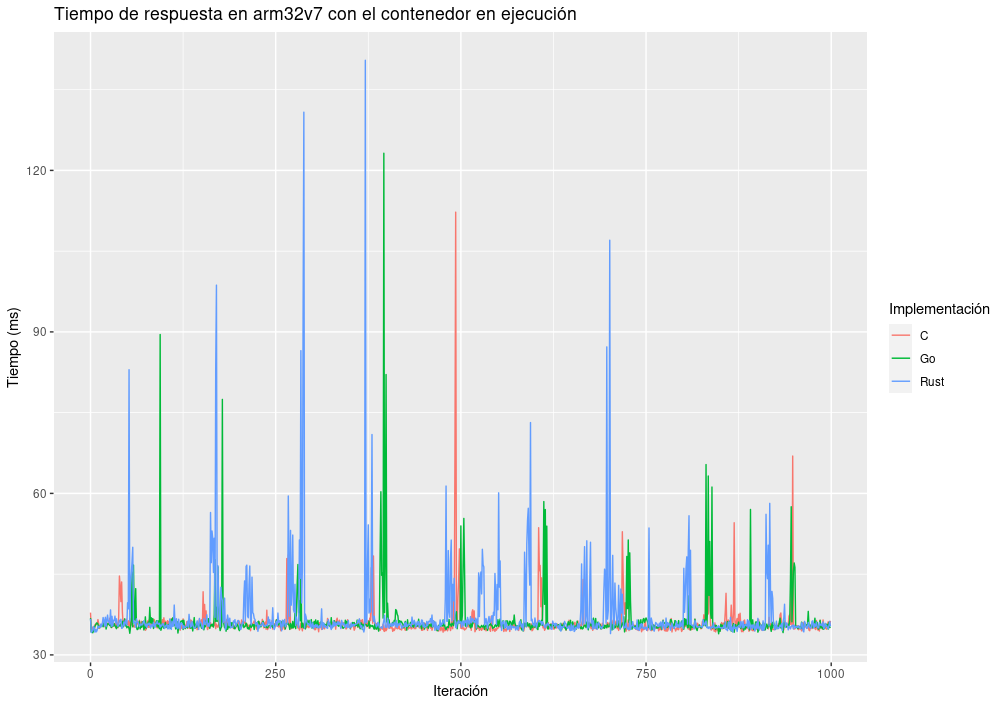
\includegraphics[width=\textwidth]{images/response-time/arm-running.png}
    \caption{Tiempos de respuesta en armv7 en ejecución}
    \label{fig:response-time-arm-running}
\end{figure}

\begin{figure}
    \centering
    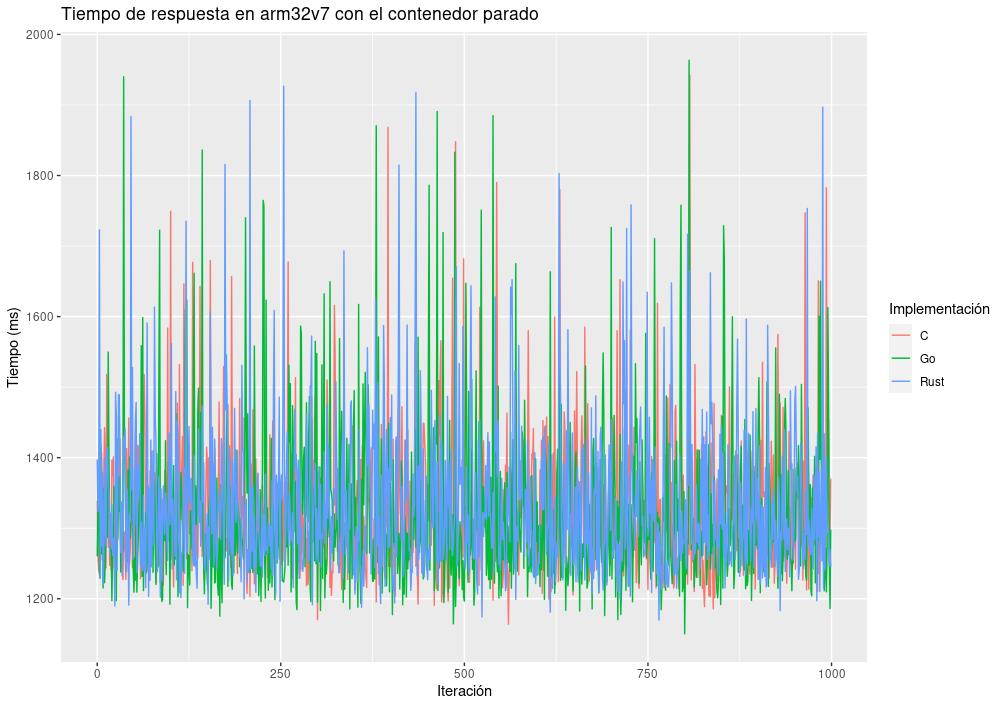
\includegraphics[width=\textwidth]{images/response-time/arm-stopped.png}
    \caption{Tiempos de respuesta en armv7 partiendo de parada}
    \label{fig:response-time-arm-stopped}
\end{figure}

\begin{figure}
    \centering
    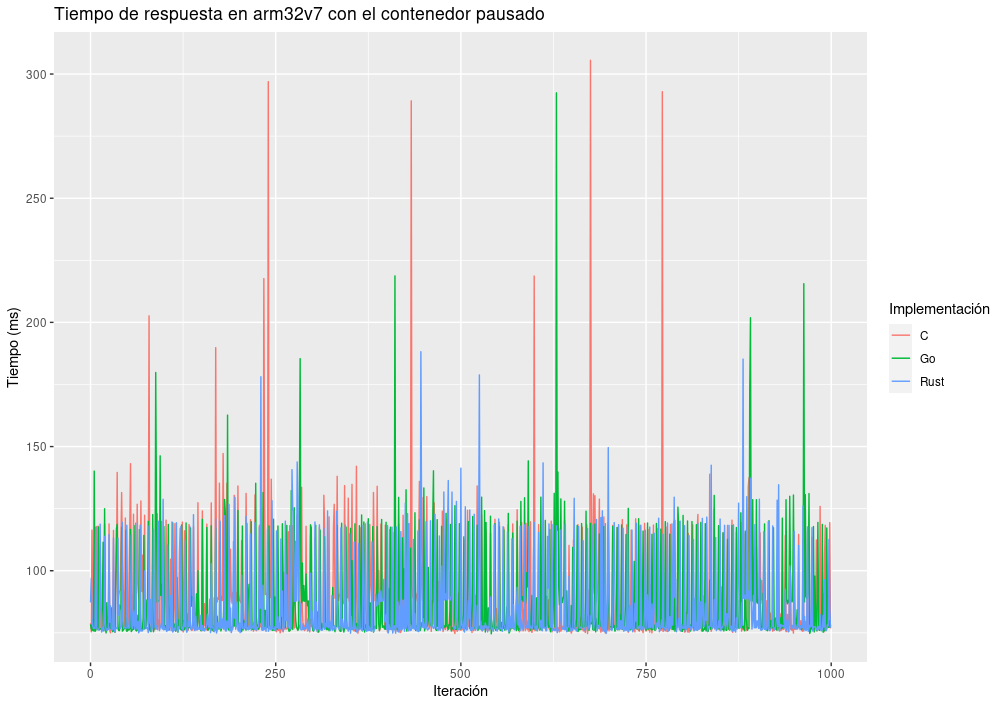
\includegraphics[width=\textwidth]{images/response-time/arm-paused.png}
    \caption{Tiempos de respuesta en armv7 partiendo de pausa}
    \label{fig:response-time-arm-paused}
\end{figure}

\newpage

Ahora, comenzamos a ver los resultados para i386, empezando por el tiempo de
respuesta con el contenedor en ejecución. La gráfica que muestra estos datos es
la de la Figura \ref{fig:response-time-i386-running}. Lo primero que destacamos
es que los tiempos son mucho más bajos y consistentes que los obtenidos en las
mismas pruebas para arm32v7, aunque se hará una comparación más detallada entre
las dos plataformas más adelante. Siguiendo con la tendencia de todas las demás
pruebas, no hay diferencias notables entre los lenguajes usados, aunque el
contenedor implementado en C es el que ha reportado más picos. Atribuir estos
picos al lenguaje sería, sin embargo, precipitado, ya que solo se producen 3 y
en solo en las primeras 500 peticiones, así que puede deberse a otras causas. En
las pruebas para el contenedor parado y pausado, cuyos tiempos se pueden ver en
las gráficas de las Figuras \ref{fig:response-time-i386-stopped} y
\ref{fig:response-time-i386-paused} respectivamente, estos tiempos son peores
que los obtenidos para arm32v7, pero siguen siendo más consistentes. Existen
algunos picos puntuales, aunque destacamos que Go es el único que no ha
presentado picos notables en ninguno de los dos casos.

\begin{figure}
    \centering
    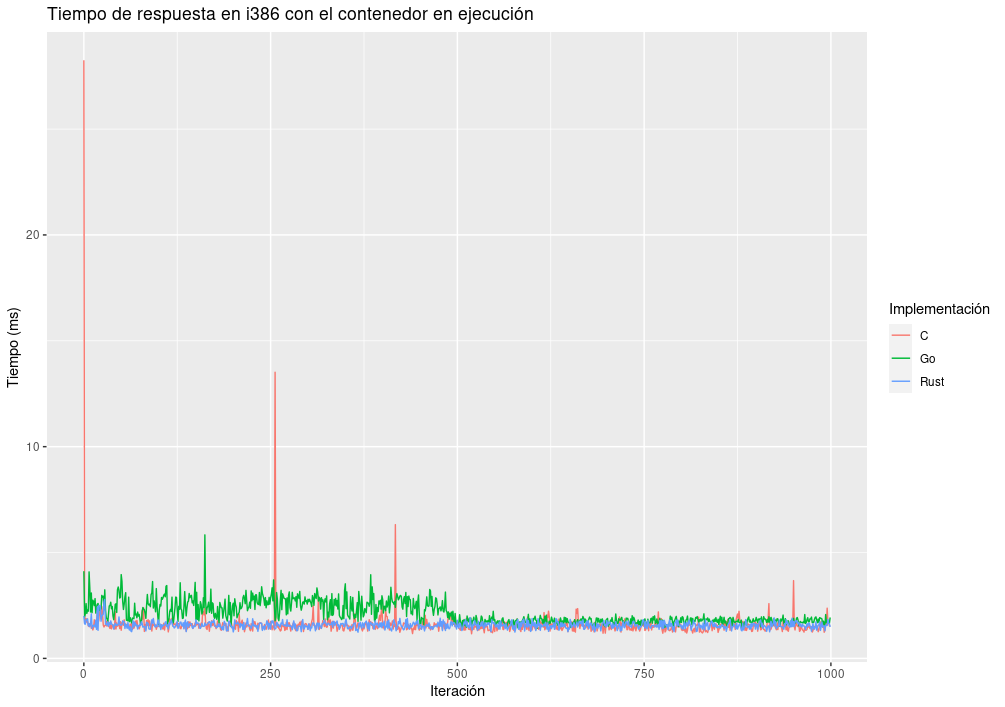
\includegraphics[width=\textwidth]{images/response-time/i386-running.png}
    \caption{Tiempos de respuesta en i386 en ejecución}
    \label{fig:response-time-i386-running}
\end{figure}

\begin{figure}
    \centering
    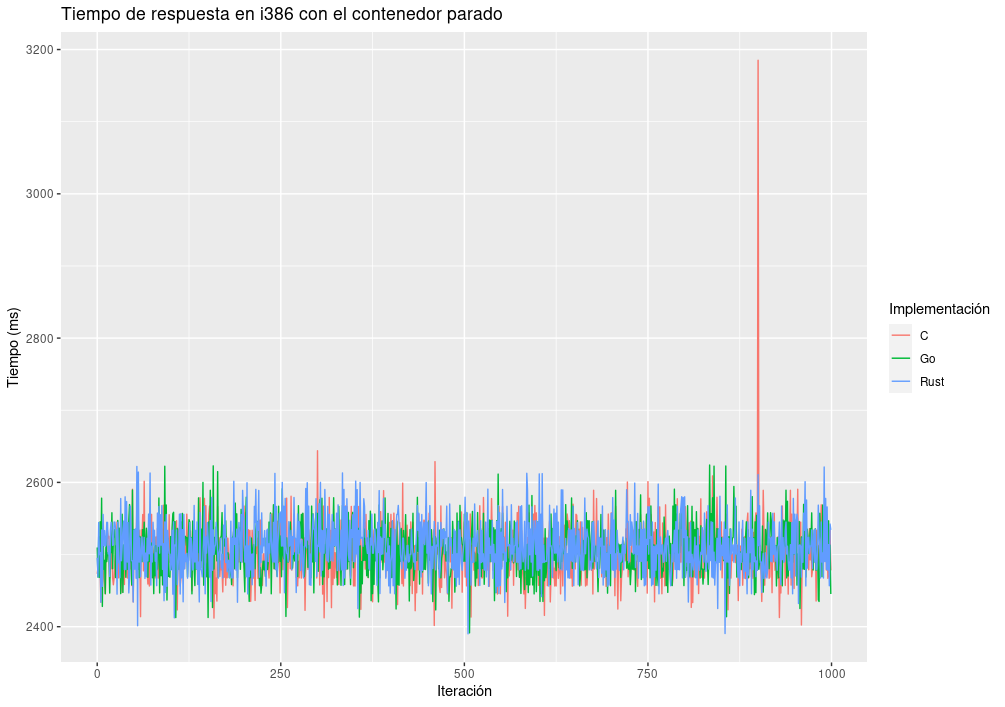
\includegraphics[width=\textwidth]{images/response-time/i386-stopped.png}
    \caption{Tiempos de respuesta en i386 partiendo de parada}
    \label{fig:response-time-i386-stopped}
\end{figure}

\begin{figure}
    \centering
    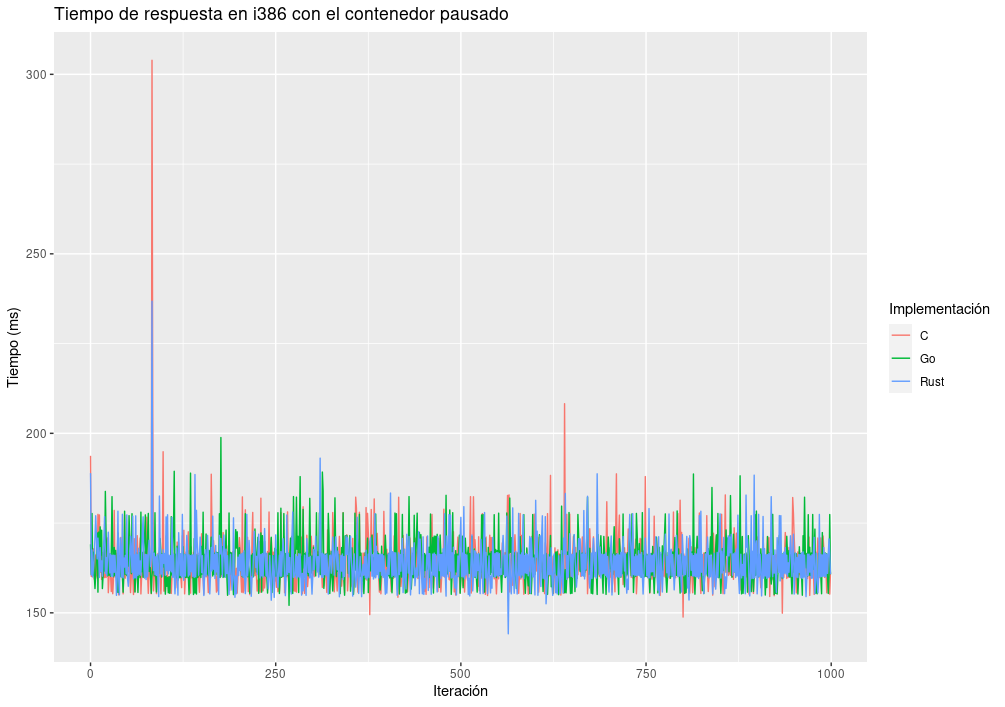
\includegraphics[width=\textwidth]{images/response-time/i386-paused.png}
    \caption{Tiempos de respuesta en i386 partiendo de pausa}
    \label{fig:response-time-i386-paused}
\end{figure}

\begin{figure}
    \centering
    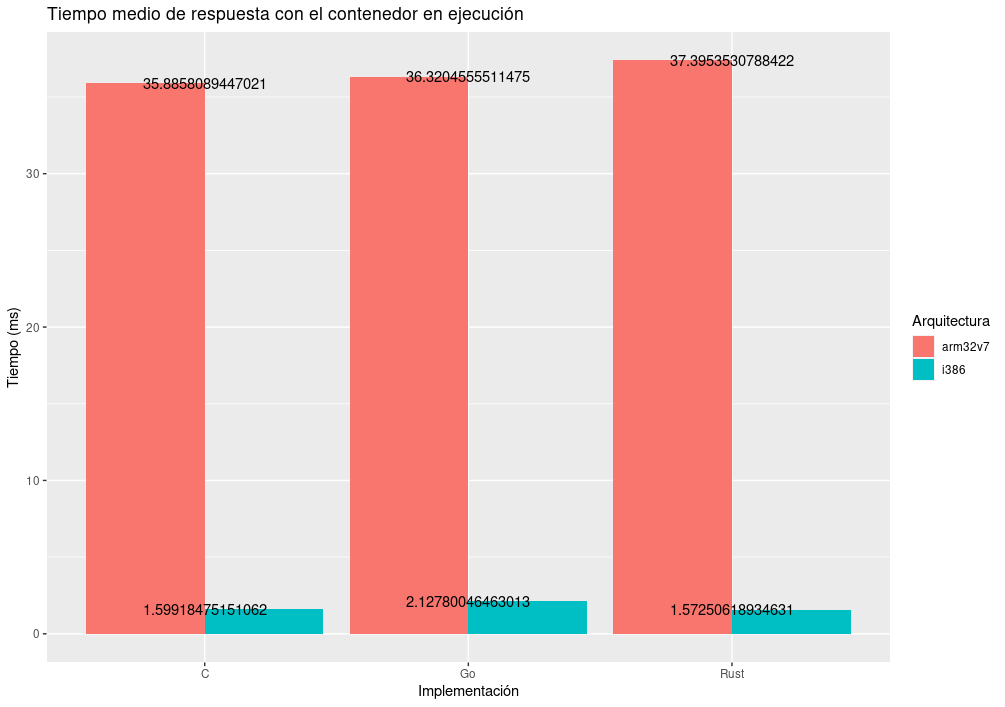
\includegraphics[width=\textwidth]{images/response-time/mean-running.png}
    \caption{Tiempos medios de respuesta en ejecución para ambas plataformas}
    \label{fig:response-time-mean-running}
\end{figure}

\newpage

Para terminar, vamos a comparar los resultados en estas pruebas para ambas
plataformas. En la Figura \ref{fig:response-time-mean-running} vemos los tiempos
medios de respuesta teniendo el contenedor en ejecución. La diferencia entre
ambas plataformas es muy grande, estando el tiempo de arm32v7 en torno a los 36
o 37 milisegundos respecto a los 2 milisegundos de media que presenta i386,
haciendo de este el único caso en el que i386 es más rápido que arm32v7. En
arm32v7, además, tenemos diferencias apreciables entre las implementaciones,
siendo Rust el lenguaje más lento y C el más rápido. En i386, Rust y C están a
la par, mientras que es Go el más lento.

Teniendo el contenedor parado, vemos en la Figura
\ref{fig:response-time-mean-stopped} que en arm32v7 los tiempos de respuesta han
sido, de media, casi la mitad de los obtenidos en i386 (en torno a 1330
milisegundos frente a 2505). En este caso, las diferencias en el tiempo son
inexistentes para los distintos lenguajes. La situación es prácticamente
idéntica cuando se tiene el contenedor pausado, obteniendo arm32v7 unos tiempos
de respuesta medios que son la mitad de los de i386, además de ser estos tiempos
casi idénticos para los 3 lenguajes usados. Los tiempos de respuesta medios para
el contenedor pausado se pueden ver en el gráfico de la Figura
\ref{fig:response-time-mean-paused}.

\begin{figure}
    \centering
    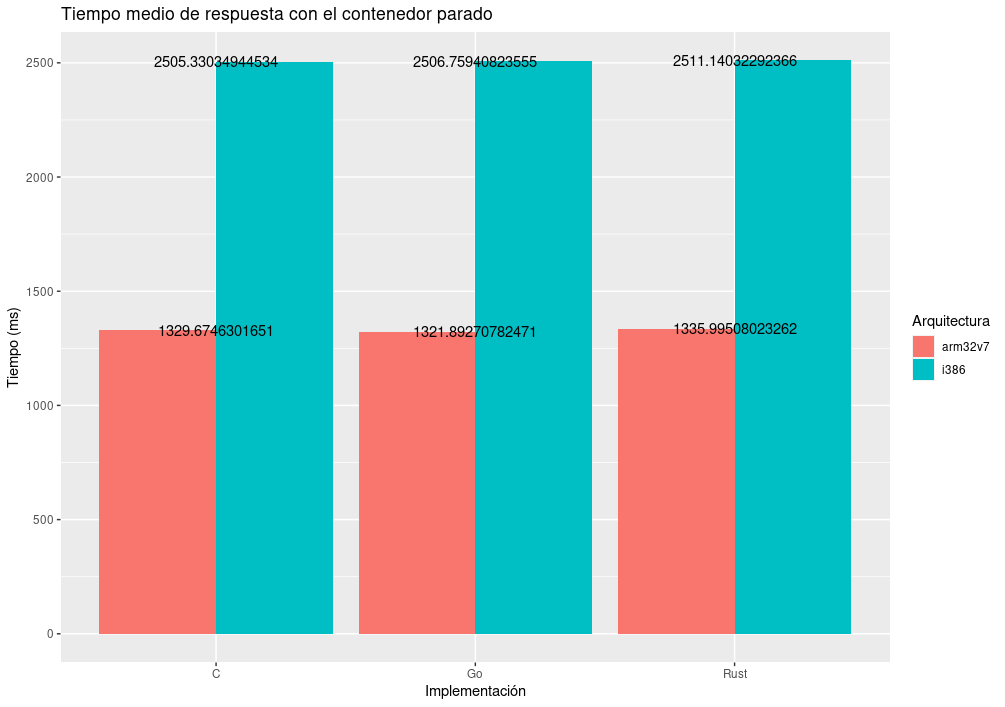
\includegraphics[width=\textwidth]{images/response-time/mean-stopped.png}
    \caption{Tiempos medios de respuesta partiendo de parada para ambas plataformas}
    \label{fig:response-time-mean-stopped}
\end{figure}

\begin{figure}
    \centering
    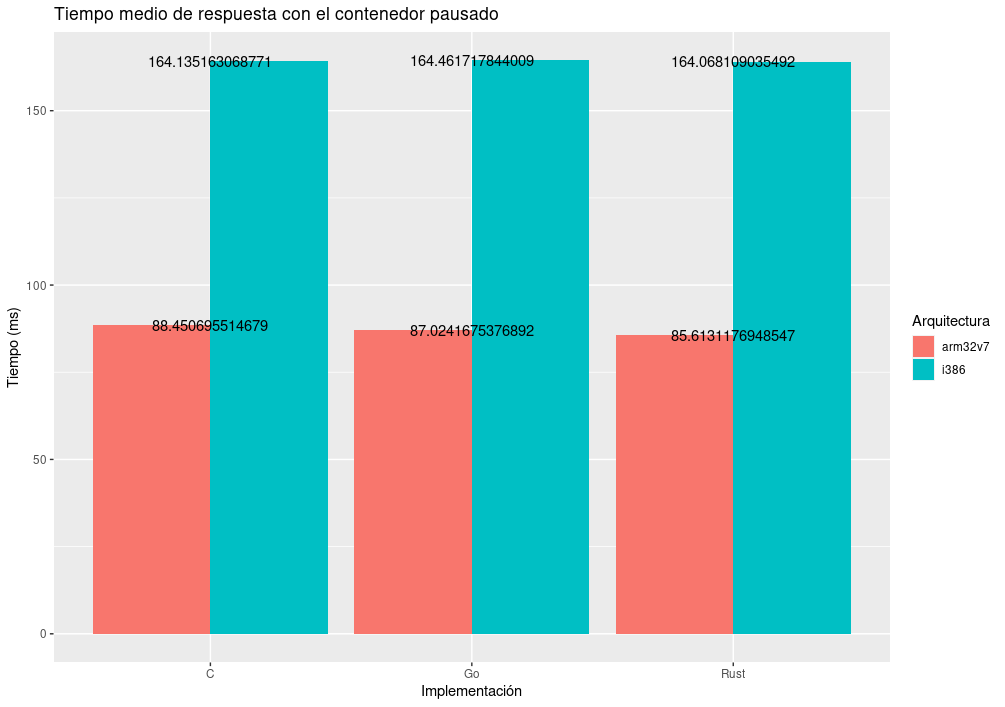
\includegraphics[width=\textwidth]{images/response-time/mean-paused.png}
    \caption{Tiempos medios de respuesta partiendo de pausa para ambas plataformas}
    \label{fig:response-time-mean-paused}
\end{figure}

\begin{figure}
    \centering
    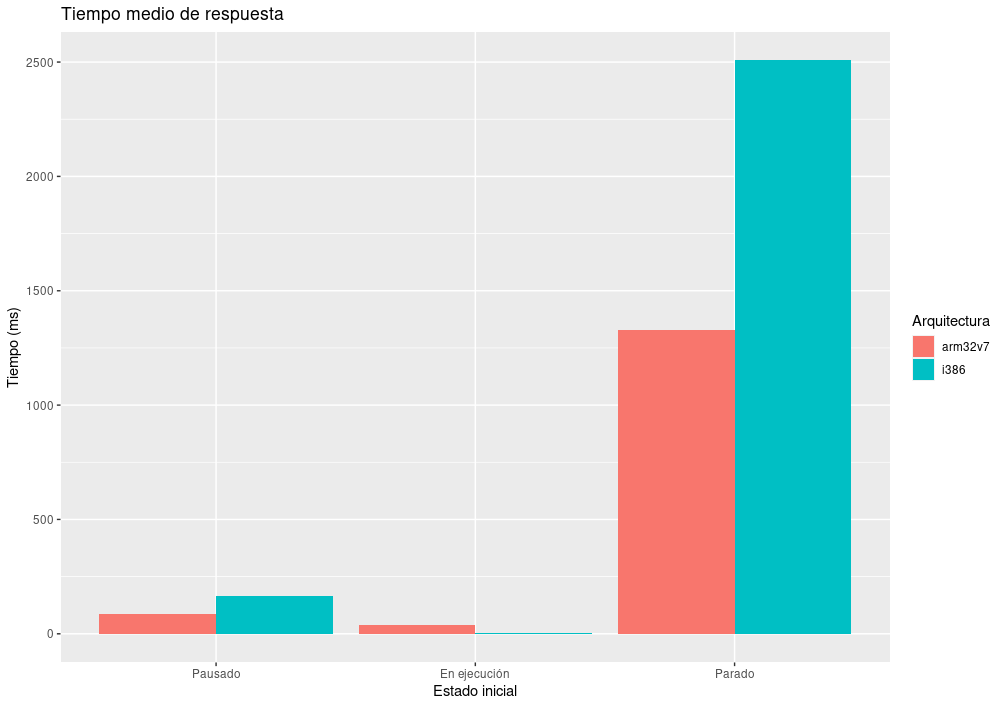
\includegraphics[width=\textwidth]{images/response-time/mean.png}
    \caption{Tiempos medios de respuesta para ambas plataformas}
    \label{fig:response-time-mean}
\end{figure}

Por último, en la Figura \ref{fig:response-time-mean} tenemos una comparativa de
los tiempos medios de respuesta para las tres situaciones y en ambas
plataformas. Esta gráfica refuerza todo lo que hemos ido indicando a lo largo de
esta subsección.
